\chapter{Tables, Figures and Matrices (oh my!)}
\label{chap-two}
In chapter \ref{chap-one} we did some typesetting and equations; now let's look at tables, figures, and matrices.

\section{Tables}
Table \ref{t:one} is about as simple as they come, to put a formula in a table just use the same methods as putting a formula in a paragraph.  Table \ref{t:two} is a similar table in landscape on a seperate page.  

\begin{table}
%per NCSU thesis editor instructions - A space needs to made between the table value and the caption, easiest way to do this is to do as shown here, add a false space by going in and out of math enviroment - JSB
\caption{$ $ Table Example}
\label{t:one}
\begin{center}
\begin{tabular}{lccl}
\hline
Treatment & No Death & Death & Total\\
Therapy A & 1295 & 72 & 1367\\
Therapy B 	& 2294 & 195 & 2489\\
Total & 3589 & 267 & 3856\\
\hline
\end{tabular}
\end{center}
\end{table}

It is important to note that LaTeX automatically tries to center everything on the page vertically so if end a page in a table or figure you may create excess space.  This template will is designed to only handle the most basic of cases, be forewarned you may need to be creative in the way you input tables and graphs for it to fit properly on the page.  
\newpage
\thispagestyle{empty}

\begin{landscape}
\begin{table}
\caption{$ $ Landscape Table Example}
\label{t:two}
\begin{center}
\begin{tabular}{lcccccccccl}
\hline
Patient & A & B & C & D & E & F & G & H &I & Total \\
\hline
John & 1 & 2 & 3 & 4 & 5 & 6 & 7 & 8 & 9 & 45 \\
Amy & 1 & 2 & 3 & 4 & 5 & 6 & 7 & 8 & 9 & 45 \\
Jim & 1 & 2 & 3 & 4 & 5 & 6 & 7 & 8 & 9 & 45 \\
Jason & 1 & 2 & 3 & 4 & 5 & 6 & 7 & 8 & 9 & 45 \\
Sandy & 1 & 2 & 3 & 4 & 5 & 6 & 7 & 8 & 9 & 45 \\
Icem & 1 & 2 & 3 & 4 & 5 & 6 & 7 & 8 & 9 & 45 \\
\hline
Total & 6 & 12 & 18 & 24 & 30 & 36 & 42 & 48 & 54 & 270\\
\end{tabular}
\end{center}
\end{table}
\end{landscape}


\section{Figures}

The easiest way to insert a picture is to have that picture in pdf format.  For this template it is somewhat crucial to use adobe acrobat to help you with the addition and manipulation of figures in your electronic thesis pdf.  If you have to put in a sideways table or figure you MUST manually add the page number to your pdf file, which you can do in acrobat.  Here is a simple example followed by a sideways figure.

$\\$
\begin{figure}[hbtp]
\centering
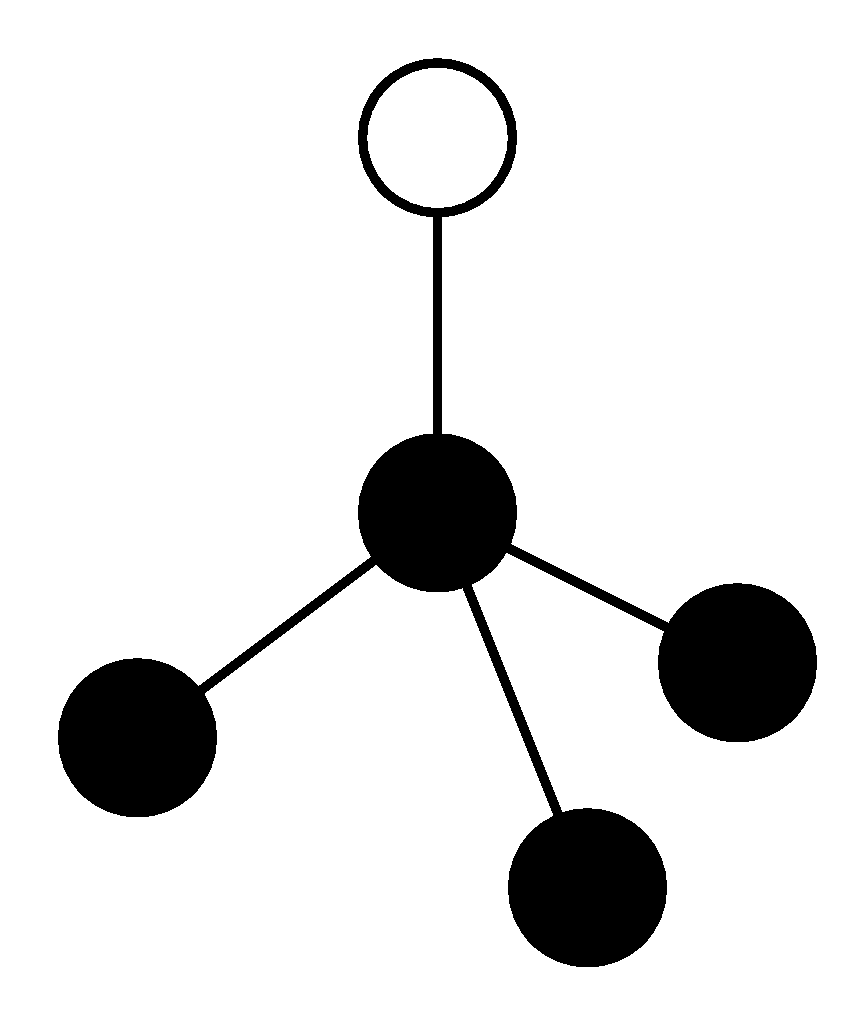
\includegraphics[width=.3\textwidth]{images/figure.pdf}
\caption{$ $ Here is a sample figure}
\label{fig-hist2}
\end{figure}
$\\$

\newpage
\thispagestyle{empty}
\begin{landscape}
\begin{figure}[hbtp]
\centering
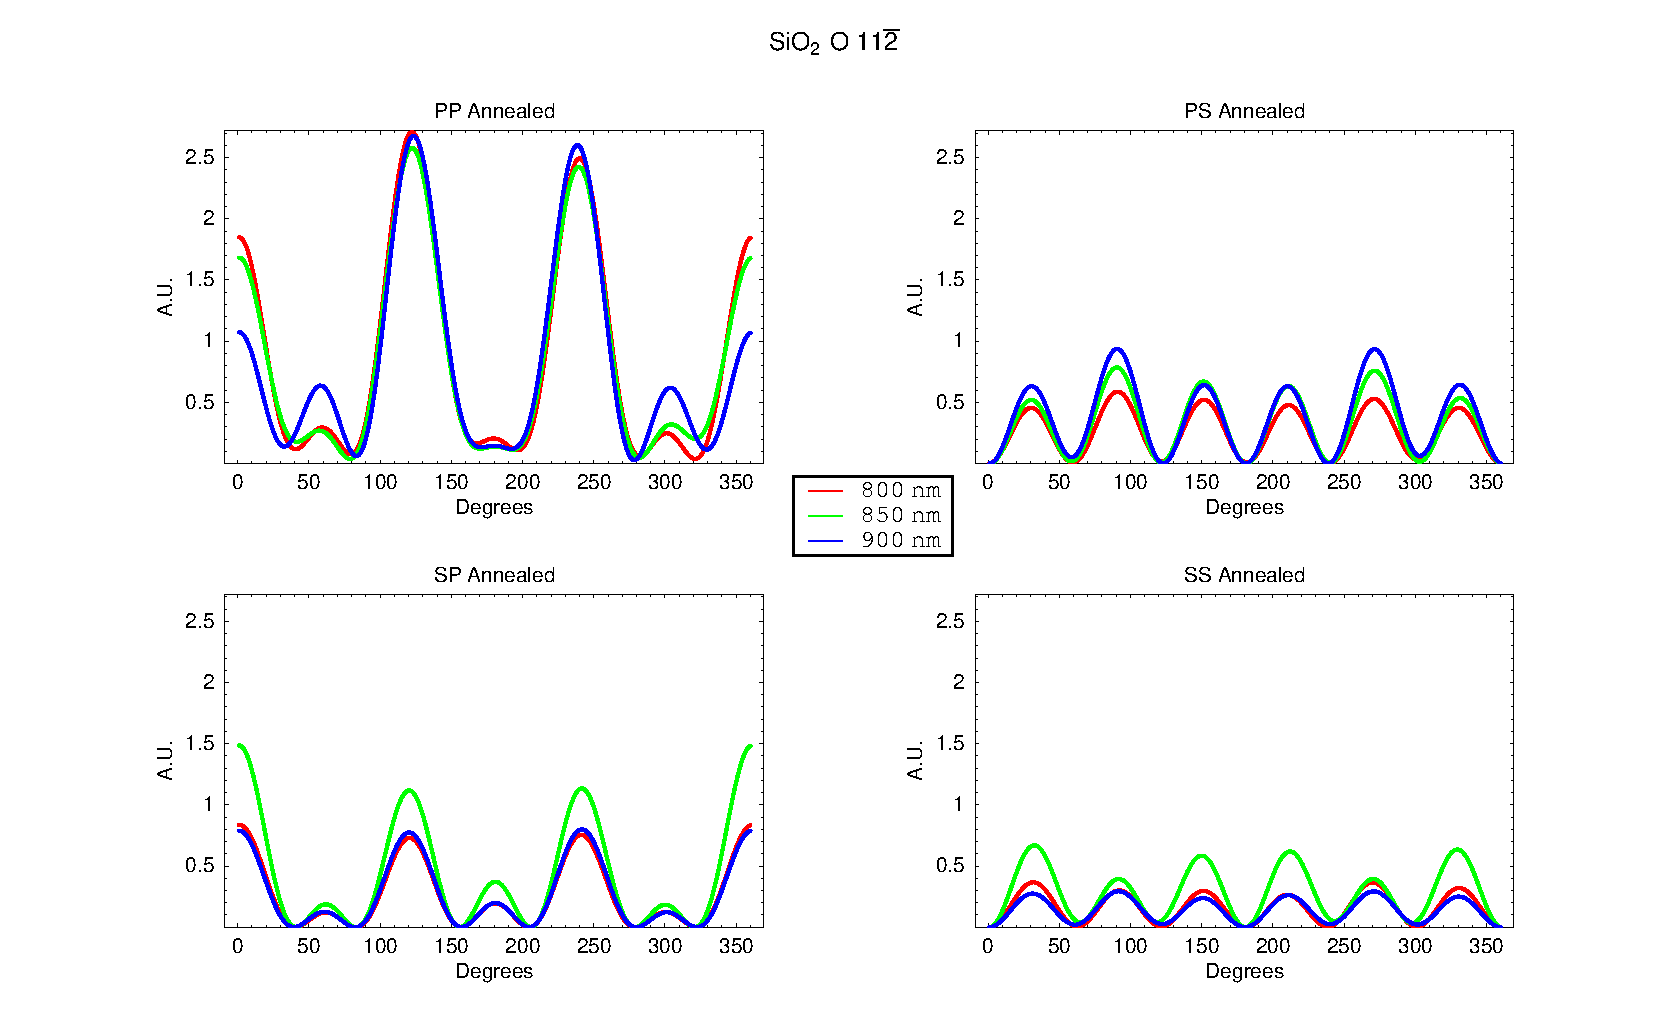
\includegraphics[width=1.3\textwidth]{images/sideways-figure.pdf}
\caption{$ $ Here is an example of a figure that has been turned sideways, need to add page numbers in adobe acrobat}
\label{fig-hist}
\end{figure}
\end{landscape}

\section{Matrices}
Let's look at a simple example of a matrix:
\[ \left( \begin{array}{ccc}
a & b & c \\
d & e & f \\
g & h & i \end{array} \right)\] 


You may prefer to write it this way:
\[ \left[\begin{array} {cccccc}
1 & 0 & 0 & 0 & 0 & 0 \\
0 & 1 & 0 & 0 & 0 & 0 \\
0 & 0 & 1 & 0 & 0 & 0 \\
0 & 0 & 0 & 1 & 0 & 0 \\
0 & 0 & 0 & 0 & 1 & 0 \\
0 & 0 & 0 & 0 & 0 & 1 \\

\end{array} \right] \]

